\documentclass[tikz,border=14pt]{standalone}
\usepackage[T1]{fontenc}
\usepackage{tgheros}
\renewcommand*\familydefault{\sfdefault}
\usepackage{pgfplots}
\pgfplotsset{compat=1.18}
\usepgfplotslibrary{fillbetween}
\usetikzlibrary{arrows.meta, calc}
\pgfdeclarelayer{background}
\pgfsetlayers{background,main}
\newcommand{\toyCliffA}{99.9000}\newcommand{\toyCliffAL}{99.9}
\newcommand{\toyCliffB}{71.5000}\newcommand{\toyCliffBL}{71.5}
\newcommand{\toyCliffC}{3.6667}\newcommand{\toyCliffCL}{3.7}
\newcommand{\toyCliffD}{1.6333}\newcommand{\toyCliffDL}{1.6}
\newcommand{\realCliffA}{84.5000}\newcommand{\realCliffAL}{84.5}
\newcommand{\realCliffB}{51.0000}\newcommand{\realCliffBL}{51.0}
\newcommand{\realCliffC}{6.5000}\newcommand{\realCliffCL}{6.5}
\newcommand{\toyAttA}{0.7122}\newcommand{\toyAttAL}{0.71}
\newcommand{\toyAttB}{0.4090}\newcommand{\toyAttBL}{0.41}
\newcommand{\toyAttC}{0.1179}\newcommand{\toyAttCL}{0.12}
\newcommand{\toyAttD}{0.0241}\newcommand{\toyAttDL}{0.02}
\newcommand{\realAttIn}{0.4632}\newcommand{\realAttInL}{0.46}
\newcommand{\realAttFar}{0.1077}\newcommand{\realAttFarL}{0.11}
\newcommand{\realHeads}{39.0000}\newcommand{\realHeadsL}{39}
\newcommand{\toyNone}{1.6667}\newcommand{\toyNoneL}{1.7}
\newcommand{\realTwoNone}{51.0000}\newcommand{\realTwoNoneL}{51.0}
\newcommand{\realFourNone}{6.5000}\newcommand{\realFourNoneL}{6.5}
\newcommand{\toyPatch}{76.1500}\newcommand{\toyPatchL}{76.1}
\newcommand{\realTwoPatch}{85.5000}\newcommand{\realTwoPatchL}{85.5}
\newcommand{\realFourPatch}{65.0000}\newcommand{\realFourPatchL}{65.0}
\newcommand{\toySham}{1.2833}\newcommand{\toyShamL}{1.3}
\newcommand{\realTwoSham}{1.0000}\newcommand{\realTwoShamL}{1.0}
\newcommand{\realFourSham}{1.0000}\newcommand{\realFourShamL}{1.0}
\newcommand{\realFourPatchFull}{25.5000}\newcommand{\realFourPatchFullL}{25.5}
\newcommand{\bestFixAnywhere}{9.3333}\newcommand{\bestFixAnywhereL}{9.3}
\newcommand{\fixMaxFar}{1.4333}\newcommand{\fixMaxFarL}{1.4}
\newcommand{\auditToyNone}{1.5833}\newcommand{\auditToyNoneL}{1.6}
\newcommand{\auditToyPatch}{75.6667}\newcommand{\auditToyPatchL}{75.7}
\newcommand{\auditTwoNone}{55.5556}\newcommand{\auditTwoNoneL}{55.6}
\newcommand{\auditTwoPatch}{100.0000}\newcommand{\auditTwoPatchL}{100.0}
\newcommand{\auditTwoN}{18.0000}\newcommand{\auditTwoNL}{18}
\newcommand{\marginOrig}{0.6780}\newcommand{\marginOrigL}{0.68}
\newcommand{\marginAudit}{1.1240}\newcommand{\marginAuditL}{1.12}


\definecolor{ink}{HTML}{0B0B0B}
\definecolor{muted}{HTML}{6B6A66}
\definecolor{gridc}{HTML}{E6E5E0}
\definecolor{band}{HTML}{F3F2EE}
\definecolor{cnone}{HTML}{52514E}
\definecolor{cpatch}{HTML}{2A78D6}
\definecolor{csham}{HTML}{008300}
\definecolor{corange}{HTML}{EB6834}
\definecolor{softblue}{HTML}{CFE1F7}
\definecolor{softgray}{HTML}{C9C8C2}

\newcommand{\pct}[1]{#1\%}

\pgfplotsset{
  /pgf/number format/assume math mode=true,
  base/.style={
    axis line style={muted, line width=0.4pt},
    tick style={muted, line width=0.4pt},
    tick align=outside,
    axis x line*=bottom, axis y line*=left,
    every tick label/.append style={font=\small, text=muted},
    label style={font=\small, text=muted},
    grid=major, major grid style={gridc, line width=0.4pt},
    title style={font=\normalsize\bfseries, text=ink},
    clip=false,
  },
}
\tikzset{
  figtitle/.style={font=\LARGE\bfseries, text=ink, anchor=north west, inner sep=0pt},
  figsub/.style={font=\normalsize, text=muted, anchor=north west, align=left, text width=17cm, inner sep=0pt, execute at begin node={\hyphenpenalty=10000\exhyphenpenalty=10000}},
  footnote/.style={font=\small, text=muted, anchor=north west, align=left, text width=17cm, inner sep=0pt, execute at begin node={\hyphenpenalty=10000\exhyphenpenalty=10000}},
  big/.style={font=\Large\bfseries, inner sep=2pt},
  lab/.style={font=\small, text=ink, inner sep=2pt},
  quiet/.style={font=\small, text=muted, inner sep=2pt},
}
\newcommand{\header}[2]{\node[figtitle] (title) at (0,0) {#1};
  \node[figsub] (sub) at ($(title.south west)+(0,-8pt)$) {#2};}

\newcommand{\px}[1]{(4.2 + 3.2*(#1 + 1.25))}
\newcommand{\pair}[4]{\node[tok] (k) at ({\px{#1} - 0.48}, #2) {key};
  \node[tok, fill=band] (v) at ({\px{#1} + 0.48}, #2) {value};
  \draw[cpatch, line width={max(0.35, 11*#3)*1pt}, line cap=round]
    ($(v.north)+(0,1pt)$) .. controls +(0,1.5) and +(0,1.5) .. ($(k.north)+(0,1pt)$);
  \node[big, text=ink, anchor=south] at ({\px{#1}}, #2 + 1.62) {#4};}
\begin{document}
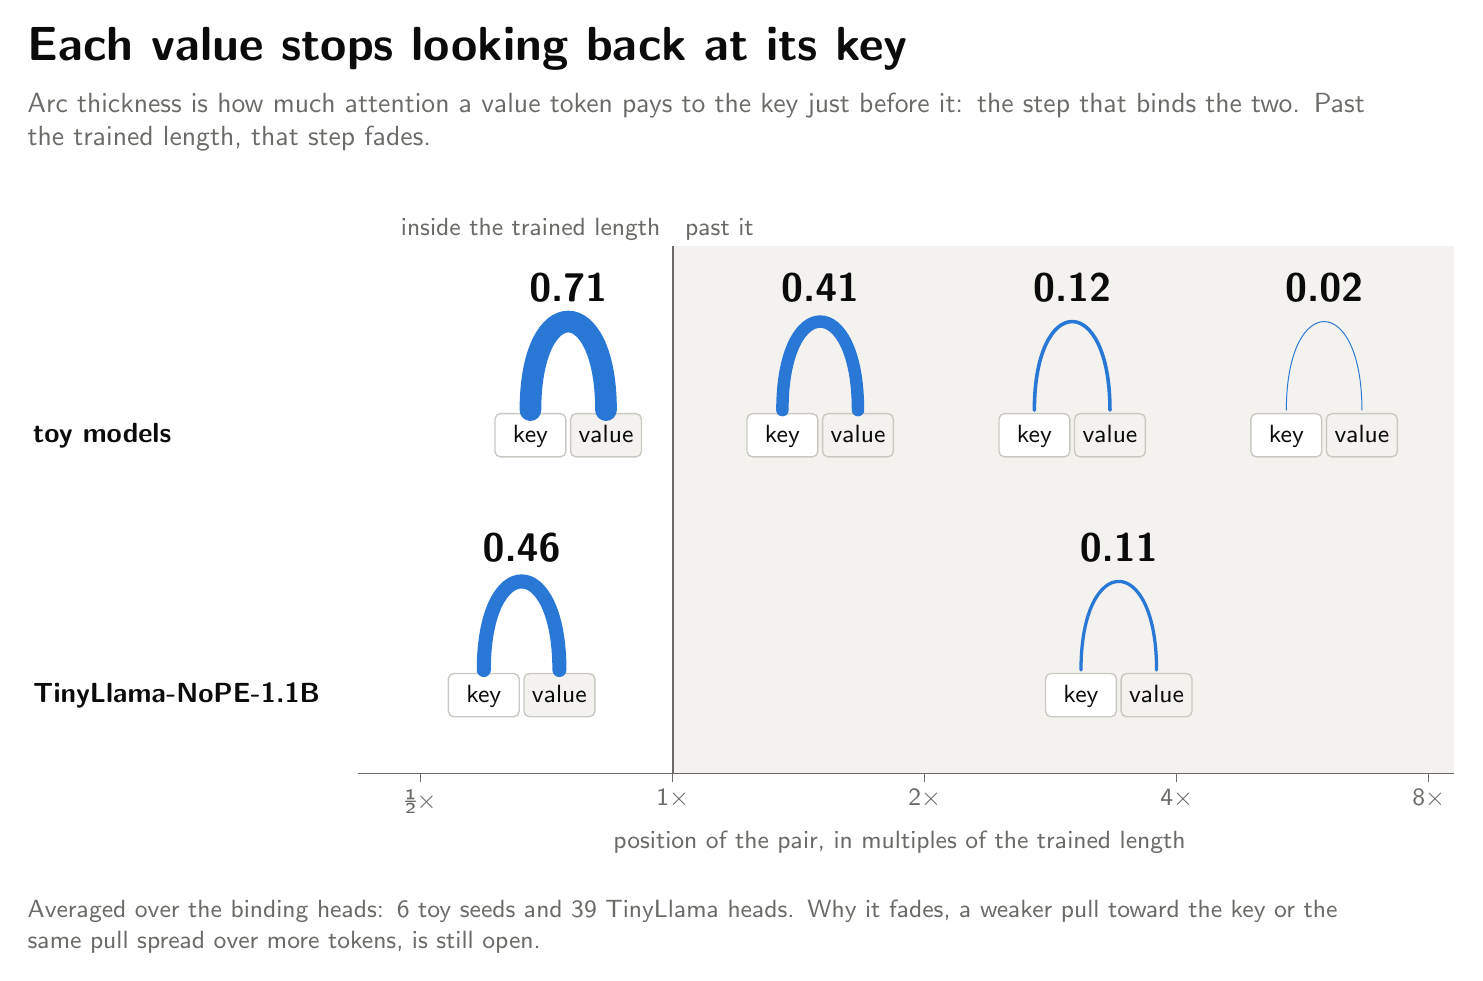
\begin{tikzpicture}[tok/.style={draw=softgray, line width=0.5pt, rounded corners=2pt, minimum width=0.9cm,
                                minimum height=0.55cm, text height=1.5ex, text depth=0.3ex, font=\small, text=ink, fill=white, inner sep=0pt}]
  \header{Each value stops looking back at its key}
    {Arc thickness is how much attention a value token pays to the key just before it: the step that binds
     the two. Past the trained length, that step fades.}

  \begin{scope}[shift={($(sub.south west)+(0,-3.6cm)$)}]
    \begin{pgfonlayer}{background}
      \fill[band] ({\px{0}}, 2.4) rectangle ({\px{3.1}}, -4.3);
    \end{pgfonlayer}
    \draw[muted, line width=0.6pt] ({\px{0}}, 2.4) -- ({\px{0}}, -4.3);
    \node[quiet, anchor=south east] at ({\px{0} - 0.08}, 2.4) {inside the trained length};
    \node[quiet, anchor=south west] at ({\px{0} + 0.08}, 2.4) {past it};
    \draw[muted, line width=0.4pt] ({\px{-1.25}}, -4.3) -- ({\px{3.1}}, -4.3);
    \foreach \l/\t in {-1/{\textonehalf$\times$}, 0/{1$\times$}, 1/{2$\times$}, 2/{4$\times$}, 3/{8$\times$}} {
      \draw[muted, line width=0.4pt] ({\px{\l}}, -4.3) -- ({\px{\l}}, -4.4);
      \node[quiet, anchor=north] at ({\px{\l}}, -4.42) {\t};
    }
    \node[quiet, anchor=north] at ({\px{0.9}}, -4.95) {position of the pair, in multiples of the trained length};

    \node[lab, font=\normalsize\bfseries, anchor=west] at (0, 0) {toy models};
    \pair{-0.415}{0}{\toyAttA}{\toyAttAL}
    \pair{0.585}{0}{\toyAttB}{\toyAttBL}
    \pair{1.585}{0}{\toyAttC}{\toyAttCL}
    \pair{2.585}{0}{\toyAttD}{\toyAttDL}

    \node[lab, font=\normalsize\bfseries, anchor=west] at (0, -3.3) {TinyLlama-NoPE-1.1B};
    \pair{-0.6}{-3.3}{\realAttIn}{\realAttInL}
    \pair{1.77}{-3.3}{\realAttFar}{\realAttFarL}
  \end{scope}

  \node[footnote] at ($(sub.south west)+(0,-9.5cm)$) {Averaged over the binding heads: 6 toy seeds and
    \realHeadsL~TinyLlama heads. Why it fades, a weaker pull toward the key or the same pull spread
    over more tokens, is still open.};
\end{tikzpicture}
\end{document}
